\appendix

\section{GPR Line of the test survey without interpretation}

\begin{figure}[H]
    \centering
    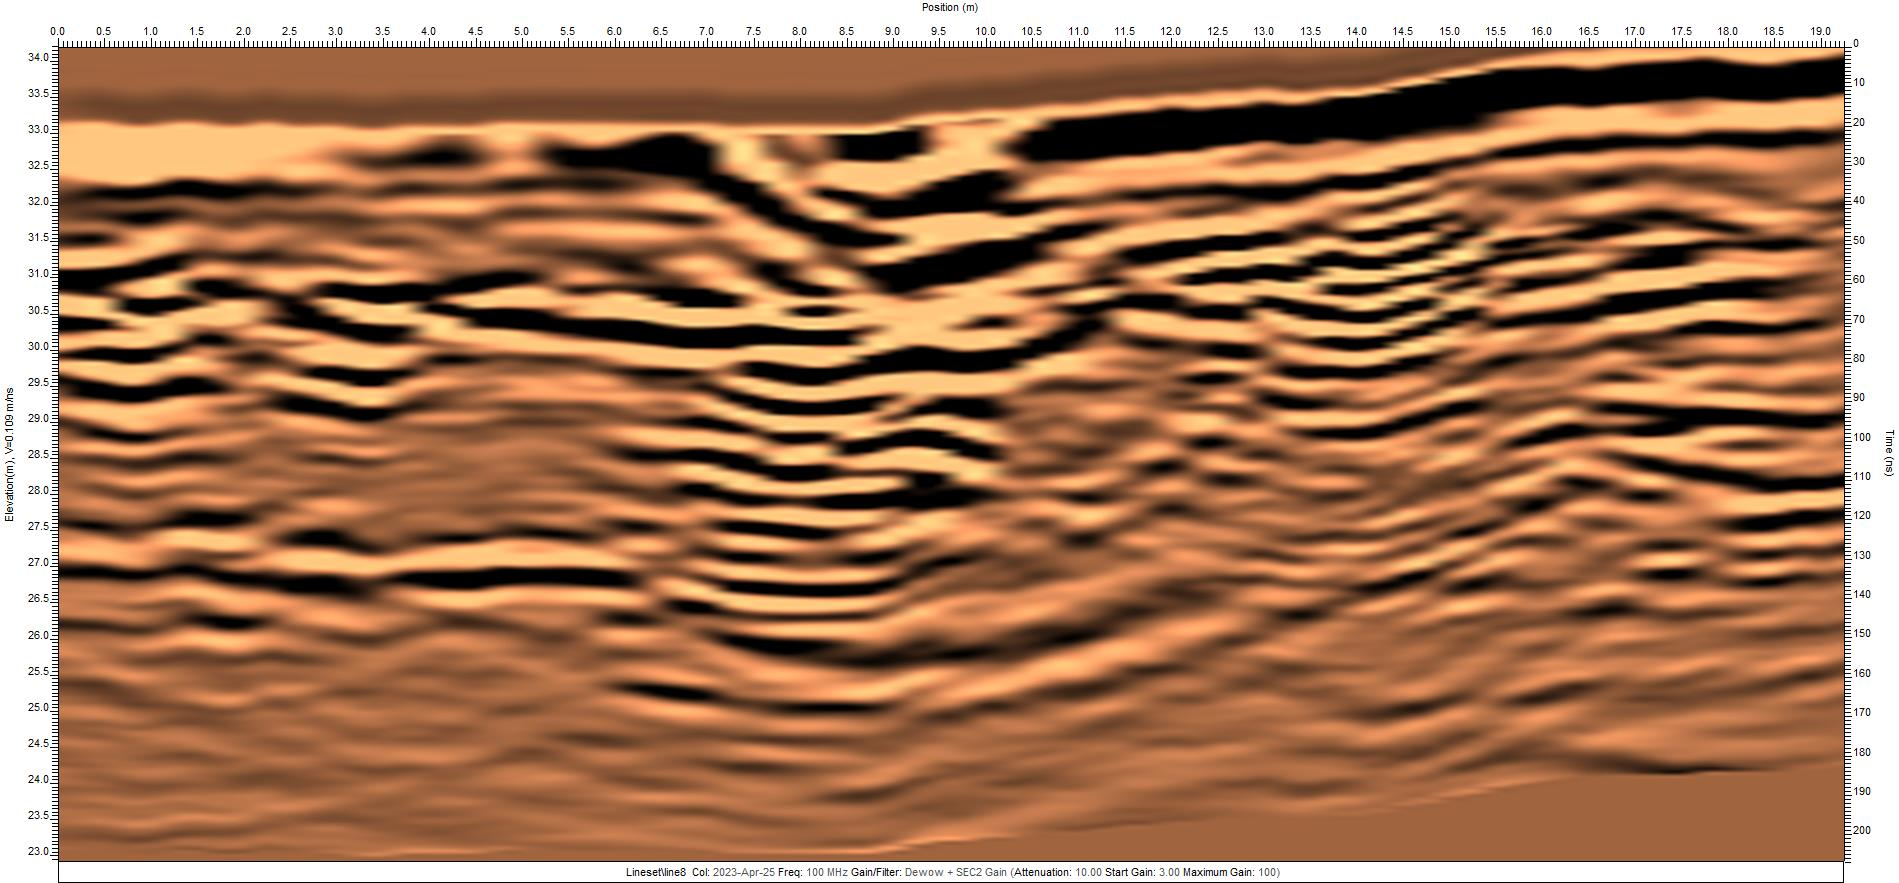
\includegraphics[width=\linewidth]{Images/00_Results/Test_line.jpg}
    \caption{Test Line}
    \label{fig:testLine_}
\end{figure}


\section{GPR Lines parallel to the slope without interpretation}

\foreach \x in {1, 16,17,18,19,21} {
    \begin{figure} [H]
        \centering
        \includegraphics[width=0.9\linewidth]{Images/00_Results/line\x.jpg}
        \caption{Line \x}
        \label{fig:line\x_}
    \end{figure}

}

\section{GPR Lines perpendicular to the slope without interpretation}

\foreach \x in {3,4,5,6,7,8,9,10,11,12,13,14,15} {
    \begin{figure} [H]
        \centering
        \includegraphics[width=0.9\linewidth]{Images/00_Results/line\x.jpg}
        \caption{Line \x}
        \label{fig:line\x_}
    \end{figure}

}